\chapter{Identify the Application Sector for your Analytic}

As stated below, this section will highlight and investigate two relevant application fields for BTS Bioengineering's gait pattern recognition analysis. An Italian motion analysis company that creates turn-key 3D Motion Capture, tri-axial Force Plate, Video and wireless \ac{emg}, hardware and software systems for research, clinical and sports. They offer quantifiable, objective data and follow the precise progress of each movement with their fully integrated systems, which measure the mechanics and dynamics of human motion.

\begin{figure}[h]
     \centering
     \begin{subfigure}[b]{0.49\textwidth}
         \centering
         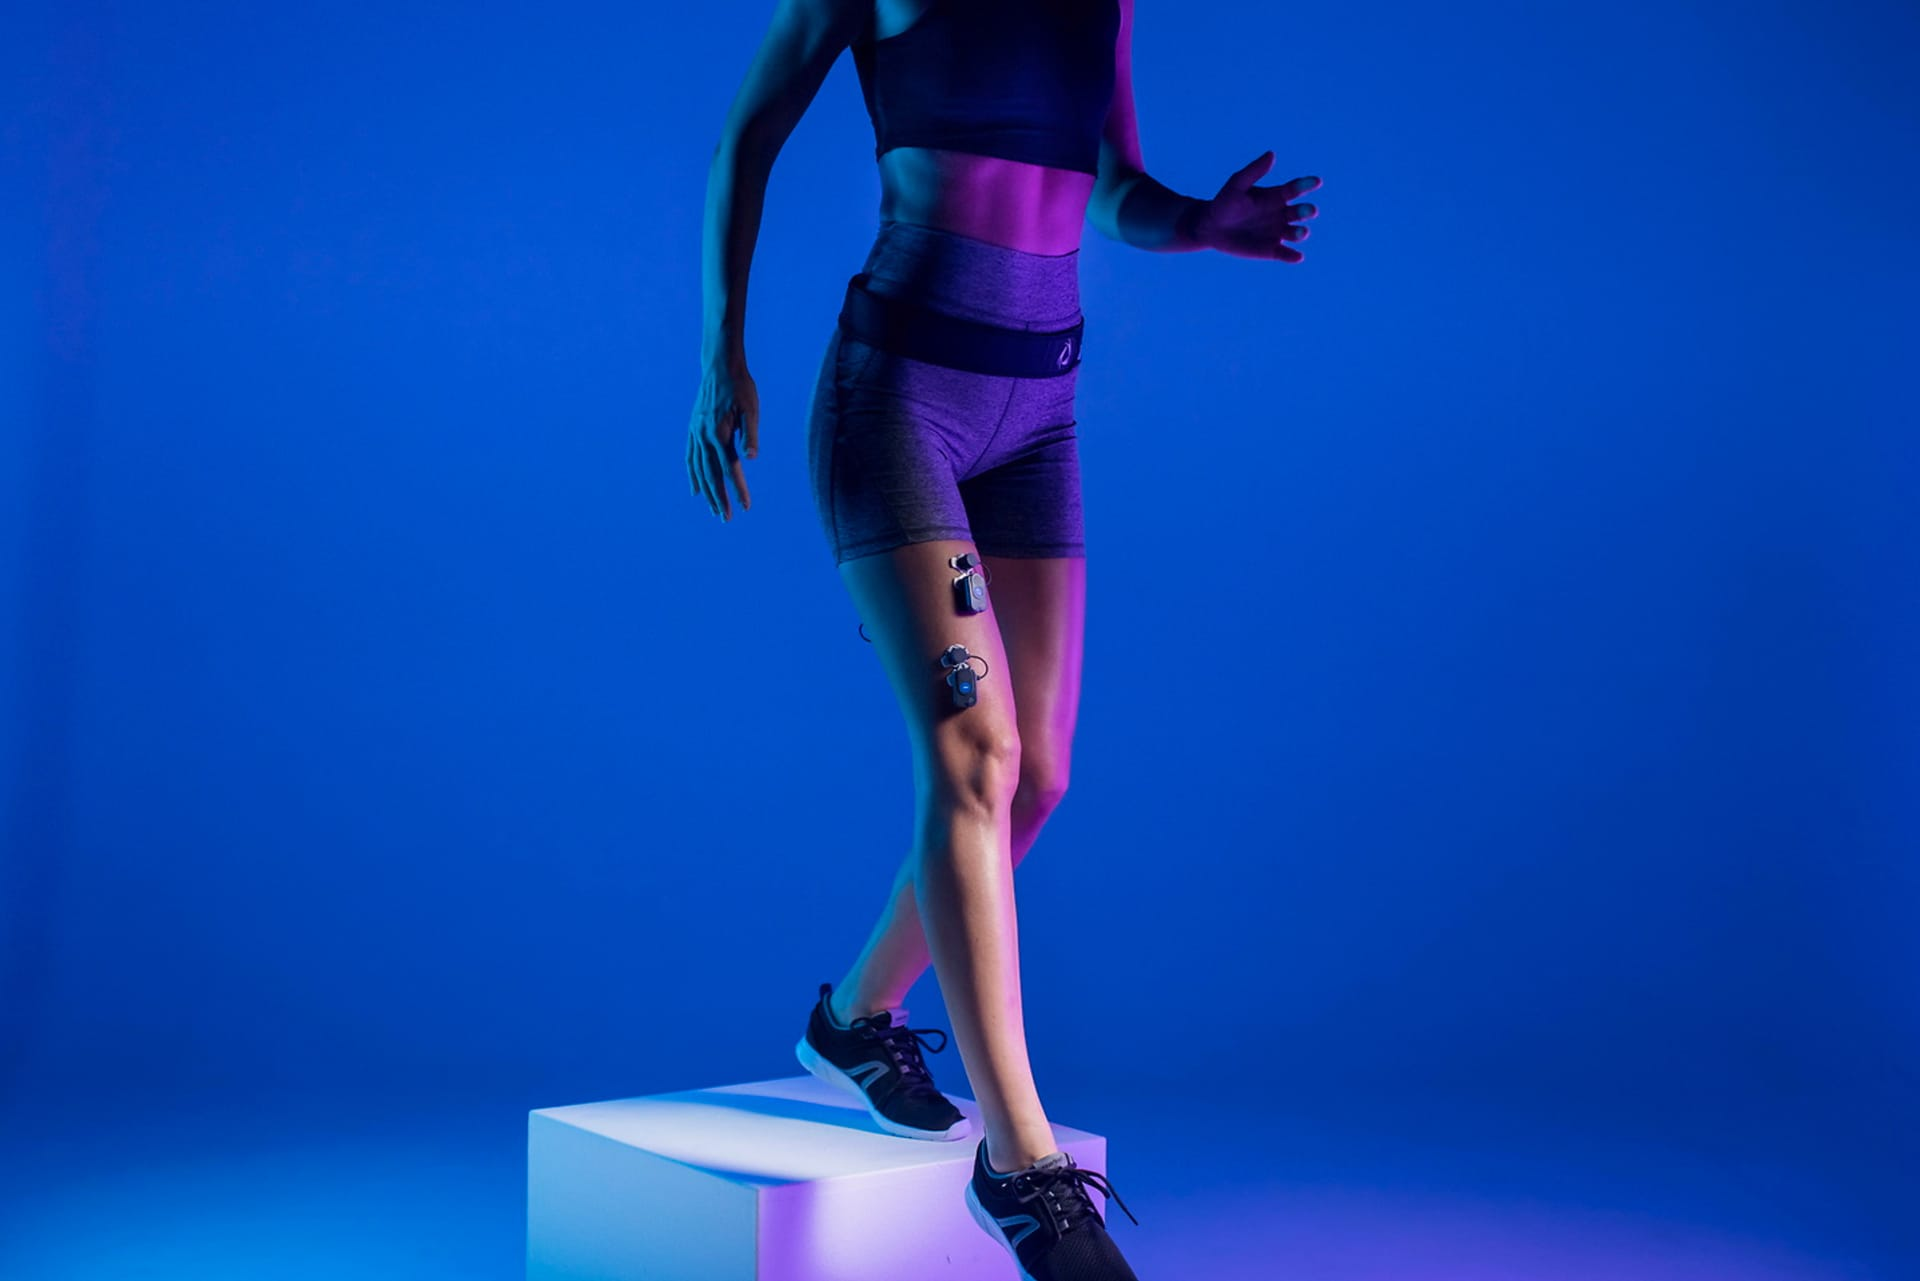
\includegraphics[scale=0.1]{Images/Injury prevention and return to play.jpeg}
         \captionsetup{justification=centering}
         \caption{Injury prevention and return to play \\ source: \cite{BTS_Injury_prevention2022}}
         \label{fig:Injury prevention and return to play}
     \end{subfigure}
     \hfill
     \begin{subfigure}[b]{0.49\textwidth}
         \centering
         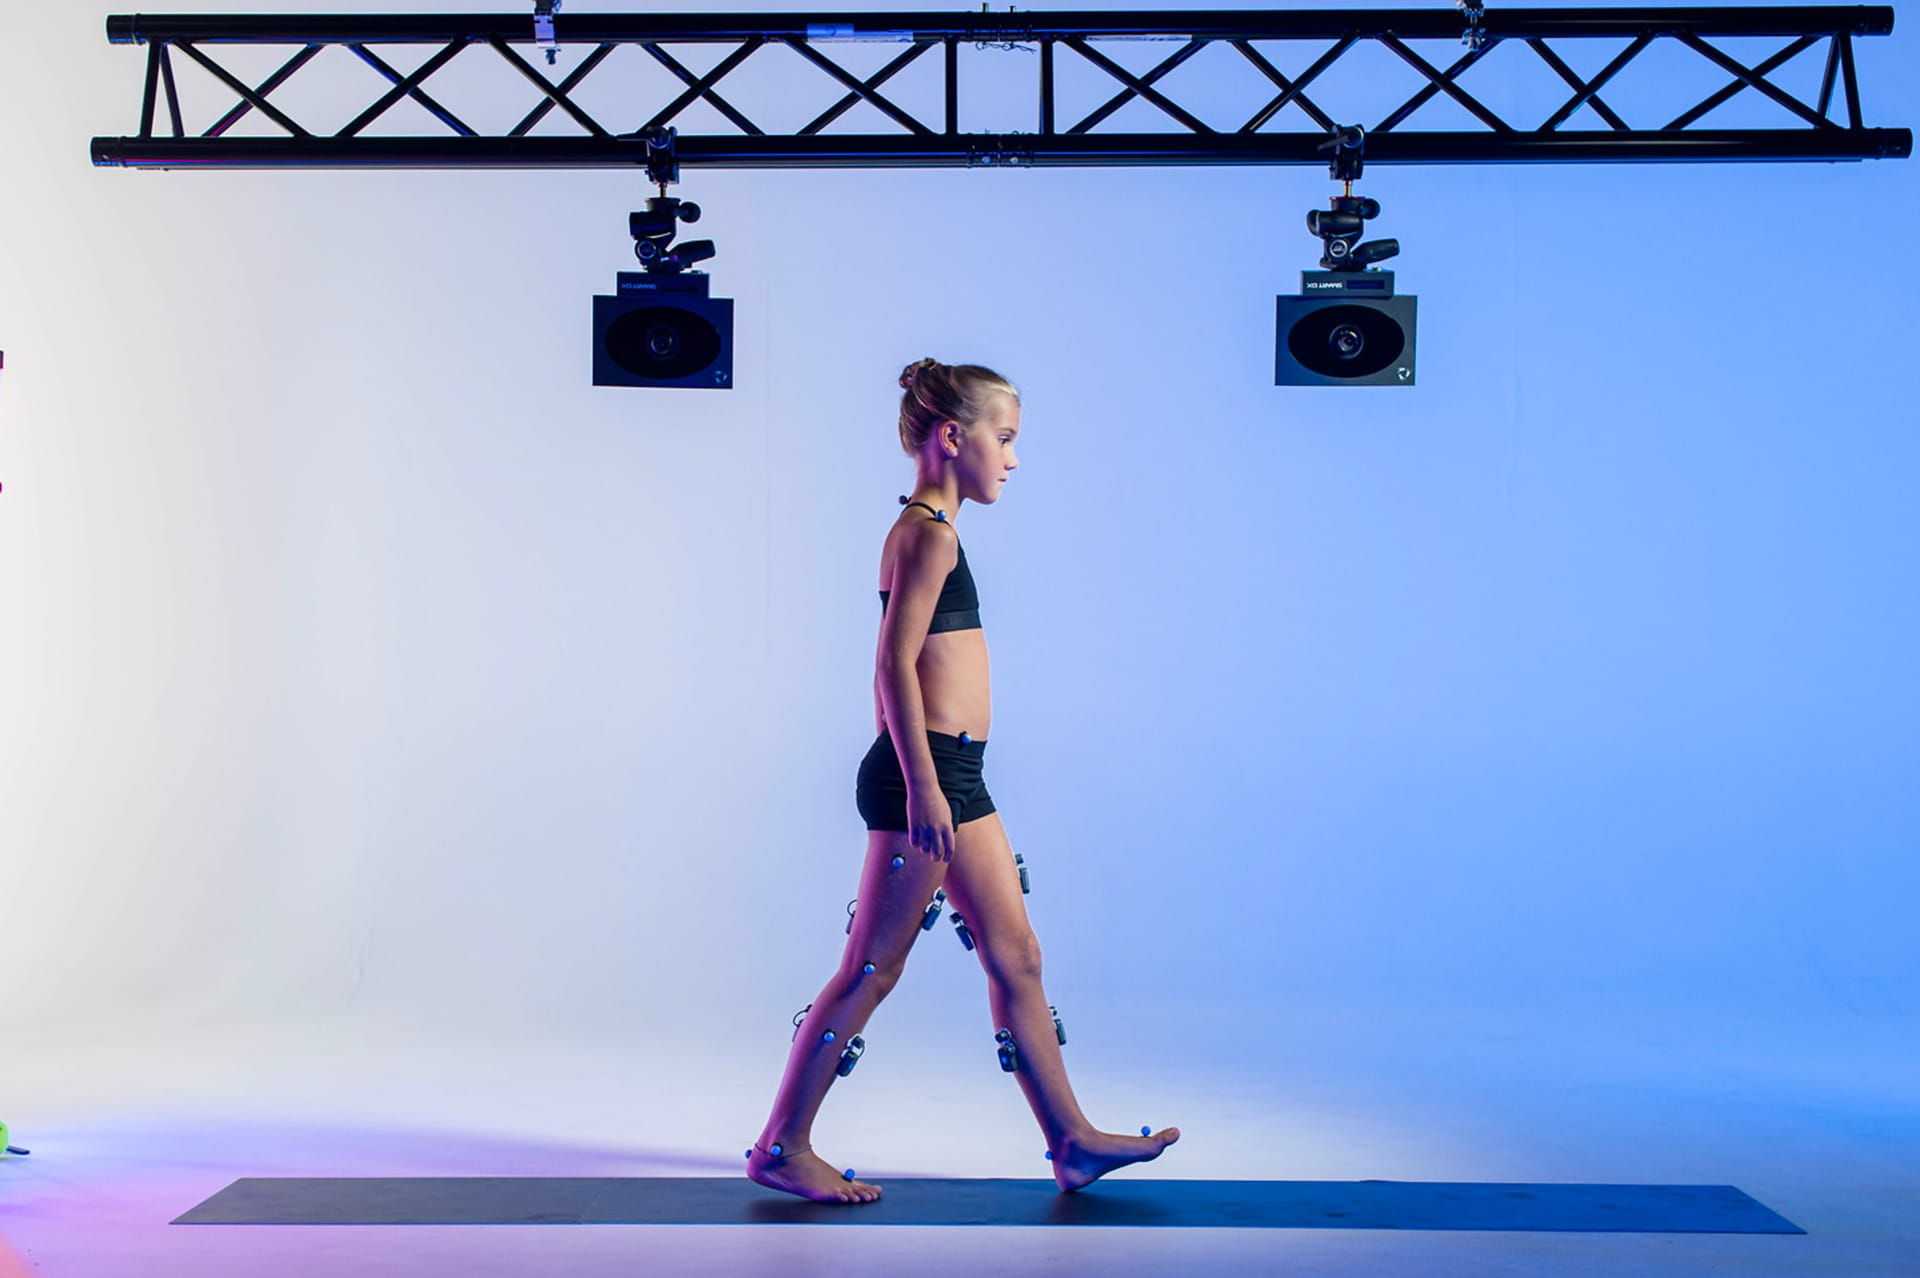
\includegraphics[scale=0.1]{Images/Evaluation and treatment of Cerebral Palsy children.jpeg}
         \captionsetup{justification=centering}
         \caption{Evaluation of Cerebral Palsy children \\ source: \cite{BTS_Carebral_palsy2022}}
         \label{fig:Evaluation and treatment of Cerebral Palsy children}
     \end{subfigure}
        \caption{BTS Bioengineering’s gait pattern recognition analysis application}
        \label{fig:BTS Bioengineering’s gait pattern recognition analysis application}
\end{figure}

\section{Injuries prevention and return to play application}

\noindent The primary goals of this application are injury prevention and the identification of optimal rehabilitation protocols in the event of injury \cite{BTS_Injury_prevention2022}. BTS Bioengineering's technologies and functional assessment tests are widely used by athletic trainers across several sports, for instance, MilanLab by AC Milan, PhysioeduLab, and Ripoll y de Prado Sport Clinic. Using their software's analysis techniques, consumers can keep tabs on the athlete's progress toward complete health and determine the best time for them to return to competitive sports. Hence, the main 3 key points of this application are indicated as follow:

\bigskip

\begin{itemize}
\item \textbf{Multiple factor assessment}:
Static and dynamic evaluation, Load analysis, Symmetries and deviation of the center of pressure
\item \textbf{Jump analysis}:
Assessment of force, speed, jump height and specific parameters
\item \textbf{Protocols for specific movements}:
Analysis of free running, treadmill running, bike fitting, total body
\end{itemize}

\section{Evaluation and treatment of cerebral palsy children application}

\noindent Patients diagnosed with infantile cerebral palsy experience stiffness and increasing muscular shortening, which contribute to dysfunction in movement patterns and make it difficult for them to move around and explore their surroundings. As a result, the key objectives of this application are to provide cutting-edge solutions for objectively evaluating children's impairments and rehabilitation using biofeedback and virtual reality \cite{BTS_Carebral_palsy2022}.Hence, the main 3 key points of this application are indicated as follow:

\begin{itemize}
\item \textbf{Monitoring}: \\
Comparison of results over time to monitor the evolution of the treatment
\item \textbf{Objective measures}: \\
Quantitative data to support clinical evaluation and to customize treatment
\item \textbf{Comparison indices}: \\
The results collected are compared with normal ranges validated by the scientific community
\end{itemize}

Because this is a non-invasive tool that respects the natural behavior of young patients, several hospitals, organizations, clinics, and universities specializing in pediatric diseases have begun to implement this application as part of their treatment protocols. Some of these establishments include the Cook Children's Medical Center, the Buzzi Foundation, the Fleni Neurology Department, and the Nio Jess University Children's Hospital.

\bigskip

The study "Evaluation of biomechanical gait parameters of patients with \ac{cp} at three different levels of gait assistance using the CPWalker" presents another use. The software delivers fast and accurate gait analysis, making it perfect for detecting issues that restrict CP patients' movement.\cite{Aycardi2019}